\documentclass{beamer}
\usepackage{charter}
\usepackage{default}
\usetheme{Madrid}
\usepackage{parskip}
\usepackage{hyperref}
%\usepackage{mathptmx}

%Information to be included in the title page:
\title{An FPGA Learning Experience: SPI Interface to Max10 FPGA}
\subtitle{ARRL and TAPR 38th Annual Digital Communications Conference}

\author{\texorpdfstring{Gregory Raven KF5N\newline\url{greg.electricity@gmail.com}}{Author}}
\date{September 21 2019}
\logo{
\includegraphics[height=1.1cm]{./graphics/tapr-logo.png}}
\begin{document}
	
	\frame{\titlepage}
	
	\begin{frame}
	\frametitle{Biography}
	Gregory Raven, first licensed novice WD5HUV in 1978.
	
	KF5N since 1980.
	
	35 Year Motorolan, entire career designing Two-way FM Radios.
	Mostly interested in Ham Radio experimenting and science.
	Residing in Florida, all of my antennas have been blown down by hurricanes or struck by lightning.
	
	NOT a professionally trained digital hardware engineer!  I am a very "Analog-RF" engineer.
	Eventually I decided learning digital was a good idea, and I attended the TAPR conference in Maryland in 2011.  Slowly going up the learning curve since then ...
\end{frame}

	\begin{frame}
	\frametitle{The Golden Age of Single Board Computers}
	
	My early introduction to "digital" was via Arduino, and later Beaglebone and Raspberry Pi.
	The so-called "Single Board Computer" or ``SBC''.
	
	I spent a couple of years working with SBCs.  This was greatly accelerated when I got my hands on ``Exploring Beaglebone, Tools and Techniques for Building with Embedded Linux'' by Derek Molloy.  Great book!
	
	\begin{figure}[h]
		\centering
		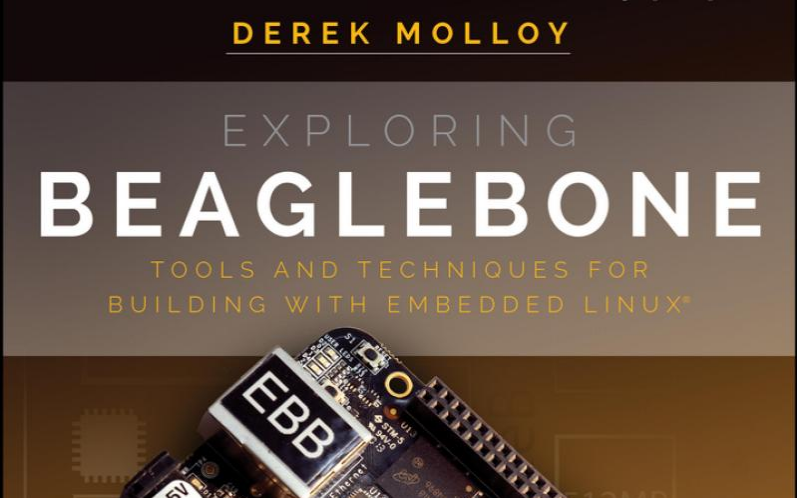
\includegraphics[width=0.75\textwidth]{graphics/beaglebone.png}
		\centering\bfseries
		\caption{``Exploring Beaglebone'' by Derek Molloy}
	\end{figure}
	
\end{frame}

\begin{frame}
\frametitle{Prerequisites to begin FPGA?}


\begin{itemize}
\item Digital Hardware experience (but not that much!)
\item Work with SBCs for a while.  Finish some projects.
\item C or similar programming.  You did this working with SBCs?
\item Discretionary time to expend.  FPGA is not rocket science, but it is time consuming!
\item Optional:  Projects with some flavor of RTOS.  Helps understanding of why FPGA is great! (ESP32, FreeRTOS, \$10)
\end{itemize}


\end{frame}

\begin{frame}
\frametitle{The State of ``Hobbyist'' FPGA}

``Hobbyist'' FPGA is miniscule compared to SBC:

\begin{itemize}
	\item Dozens, maybe hundreds of SBC books.  FPGA: 4
	\item Fair representation on hackster.io and hackaday.io.
	\item ARRL bookstore: lots of Arduino, RPi, nothing on FPGA.
\end{itemize}

As usual, Amateur Radio experimenters were pioneers in new technology, having used FPGA to create early state-of-the-art ``Software Defined Radio'' transceivers.  This goes back to at least the early 2000s, and perhaps years earlier than that.  Does anyone know the first Amateur Radio application of FPGA? 

\end{frame}

\begin{frame}
\frametitle{FPGA Boards?}

What is out there to work with?

\url{https://makezine.com/comparison/boards/}

Currently, most FPGA are ``development boards'' intended for industrial or academic applications.

There is a little bit of good news!  Will return to this topic later ...

\end{frame}

\begin{frame}
\frametitle{What is exciting about FPGAs?}

``3-D Printer for Electronics?''

HARDWARE not software!

This gives you the power to create multiple specifically targeted digital machines which can work independently of one another.  This is the capability that SDR uses to crunch DSP math very efficiently while handling data flow simultaneously.  A list of FPGA applications from Wikipedia:

\url{https://en.wikipedia.org/wiki/Field-programmable_gate_array}

\end{frame}

\begin{frame}
\frametitle{How Do You Begin?}

For FPGA this is not as clear as SBCs.  To an SBC beginner I would say to get an Arduino UNO and a good book or website and get going.  Later graduate to embedded Linux and RPi, Beaglebone, or equivalent.

So I will give an example here, not correct for everyone ...
Lectures by Bruce Land of Cornell University using PIC32:

\begin{tiny}
\url{https://www.youtube.com/watch?v=FYy6JN0vpg0&list=PLKcjQ_UFkrd4z2qoFuJ1jtVhCSuxxCTpk}
\end{tiny}

This course uses a PIC32 microcontroller board.  However, the material in the lectures is generic enough to apply to any board which can be programmed in C.
Even better, a second course covers FPGA!

\begin{scriptsize}
\url{https://www.youtube.com/playlist?list=PLKcjQ_UFkrd7UcOVMm39A6VdMbWWq-e_c}
\end{scriptsize}

and the matching website:

\url{http://people.ece.cornell.edu/land/courses/ece5760/}

\end{frame}

\begin{frame}
\frametitle{Online MOOC Style Courses?}

I tried:

\begin{itemize}
	\item Coursera
\item Udemy
\item Hackster.io
\end{itemize}

I didn't get much out of the above.  They didn't really follow through to a practical application.  Hopefully some new courses on FPGA will appear, and I'm sure they will.
So far my experience with FPGA MOOCs is underwhelming.

\end{frame}

\begin{frame}
\frametitle{Better than MOOCs:  Your Friendly FPGA Device Supplier}

\begin{figure}[h]
	\centering
	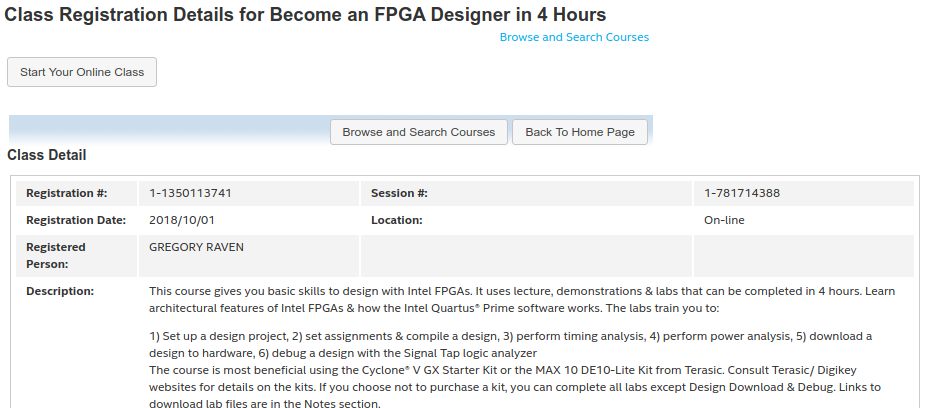
\includegraphics[width=1.0\textwidth]{graphics/fpga_designer_in_4hours.png}
	\centering\bfseries
	\caption{Intel "Become an FPGA Designer in 4 Hours"}
\end{figure}

\end{frame}



\begin{frame}
\frametitle{Choosing a Development Board}

As mentioned earlier, the choice is limited compared to SBCs.  Most are targeted at  industrial/academic application.  Many are expensive!

The Cornell FPGA course uses an "SOC" style device, and the board cost is \$250.
For someone who is not sure about FPGA, that is too much!

Also, an ``SOC'' is too much for a beginner.  This has two Cortex A9 processors, runs its own flavor of embedded Linux, and it looks overwhelming!

The same company making the DE1-SOC also makes others:

{\tiny \url{https://www.terasic.com.tw/cgi-bin/page/archive.pl?Language=English&CategoryNo=163}}

\end{frame}

\begin{frame}
\frametitle{What I Selected}

Terasic DE10-Lite is a cost-effective Altera MAX 10 based FPGA board. The board utilizes the maximum capacity MAX 10 FPGA, which has around 50K logic elements(LEs) and on-die analog-to-digital converter (ADC). It features on-board USB-Blaster, SDRAM, accelerometer, VGA output, 2x20 GPIO expansion connector, and an Arduino UNO R3 expansion connector in a compact size.

The DE10-Lite kit also contains lots of reference designs and software utilities for users to easily develop their applications based on these design resources.

{\tiny
\url{https://www.terasic.com.tw/cgi-bin/page/archive.pl?Language=English&CategoryNo=234&No=1021}}

\end{frame}

\begin{frame}
\frametitle{What I Selected}

\begin{figure}[h]
	\centering
	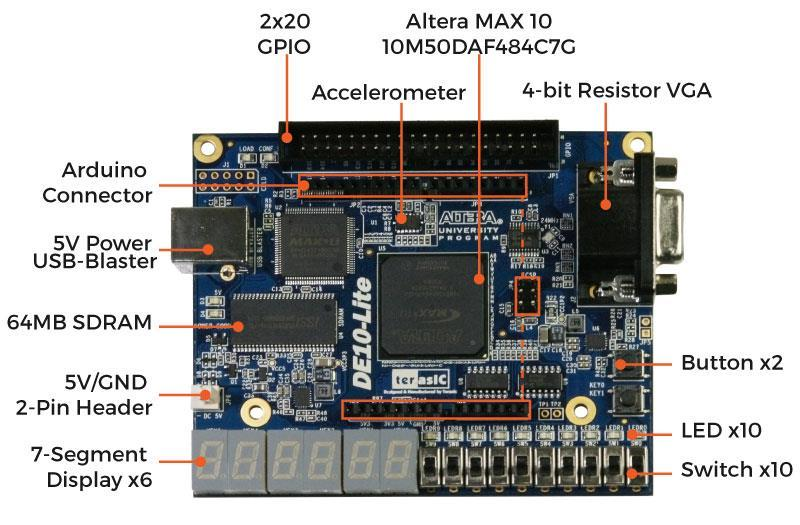
\includegraphics[width=0.9\textwidth]{graphics/de10-lite.jpg}
	\centering\bfseries
	\caption{Terasic DE10-Lite \$85}
\end{figure}

\end{frame}

\begin{frame}
\frametitle{Wait!!! Don't Put it in the Cart and Purchase}

This is not a moment for ``instant gratification''!  You have some work to do first.

Before you take the plunge, you MUST install the tools required to make this thing work!
I chose an Intel (formerly Altera) based board (MAX10), so this means installing ``Quartus''.  Xilinx devices will require ``Vivado''.

But to do this, you should get a ``free'' account at the Intel site:

\url{https://www.intel.com/content/www/us/en/products/programmable.html}

Go here for ``Quartus Prime Lite'':

\url{http://fpgasoftware.intel.com/?edition=lite}

Make sure you can install and run this large beast!

\end{frame}

\begin{frame}
\frametitle{Development Platforms}

I am a huge fan of Linux and I almost always use a distribution of Ubuntu.
Quartus has a version for Windows, however, I have not tested it.

Regarding Ubuntu, I don't recommend running Quartus in Ubuntu directly.  The simulation tool, Vsim, will not run.

Instead, use a Virtual Box to create a ``virtual machine''.  I experimented with Centos 6 and 7.  Centos 6 was the easiest to configure.

Quartus is a significant user of desktop real estate.  I don't think anything less than full HD (1920x1080) is going to be satisfactory.  I found FHD to be marginal, and I bought a new 27 inch ``QHD'' display, which is 2560x1440 pixels.  Much better!

\end{frame}

\begin{frame}
\frametitle{Project Inspiration:  JTAG Interface to DE10-Lite}

I had abandoned the SOC with embedded Linux as too complex, however, I still wanted a means of ``talking'' to the FPGA, preferably from my Ubuntu box.

After a bunch of searching, I found this:

\url{https://github.com/hildebrandmw/de10lite-hdl}

The interesting feature of this project is the usage of the USB to load data (animated GIF image file) to
the FPGA. So this is a data pipeline from a Linux desktop to the FPGA which is built into the board!
The interface is via “JTAG”, which is typically used as a debugging interface. It is not specifically intended
for mass data transfer, but in this case it was pressed into service.

\end{frame}

\begin{frame}
\frametitle{Project Inspiration:  JTAG Interface to DE10-Lite}

\begin{figure}[h]
	\centering
	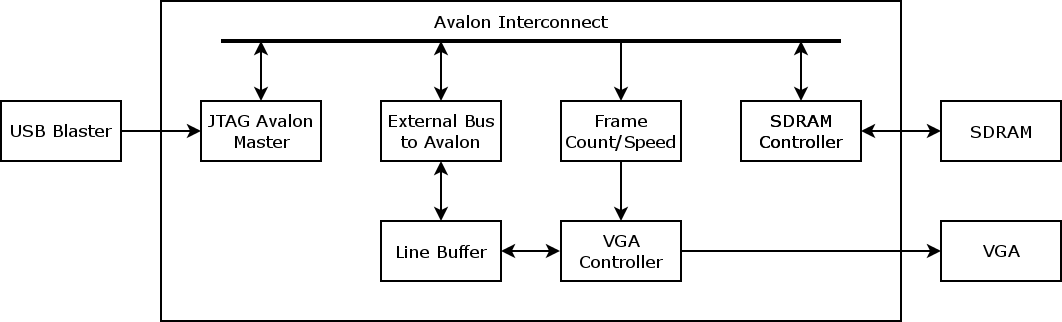
\includegraphics[width=1.0\textwidth]{graphics/play_gif.png}
	\centering\bfseries
	\caption{Play\_gif JTAG Interface System Diagram}
\end{figure}

Not shown is a running instance of Quartus and TCL/JTAG server required to make this system function.

\end{frame}

\begin{frame}
\frametitle{IP and Platform Designer}

FPGA Jargon:  ``Intellectual Property'' or ``IP''

``Intellectual Property'' (IP) in the context of semiconductor devices is a block of circuitry which has been heavily engineered and refined to perform some particular function.

Due to the way integrated circuits are manufactured, blocks of ''IP'' can be added to the silicon and be expected to perform to the IP owner's specifications.  Typically IP can be included as part of a design kit, or it can be paid for with a license fee.

In our case, we are given a whole bunch of IP for free that we can experiment with!  This is bundled into ``Platform Designer'' which is a tool-within-a-tool in the Quartus design suite.

\end{frame}

\begin{frame}
\frametitle{IP and Platform Designer}

\begin{figure}[h]
	\centering
	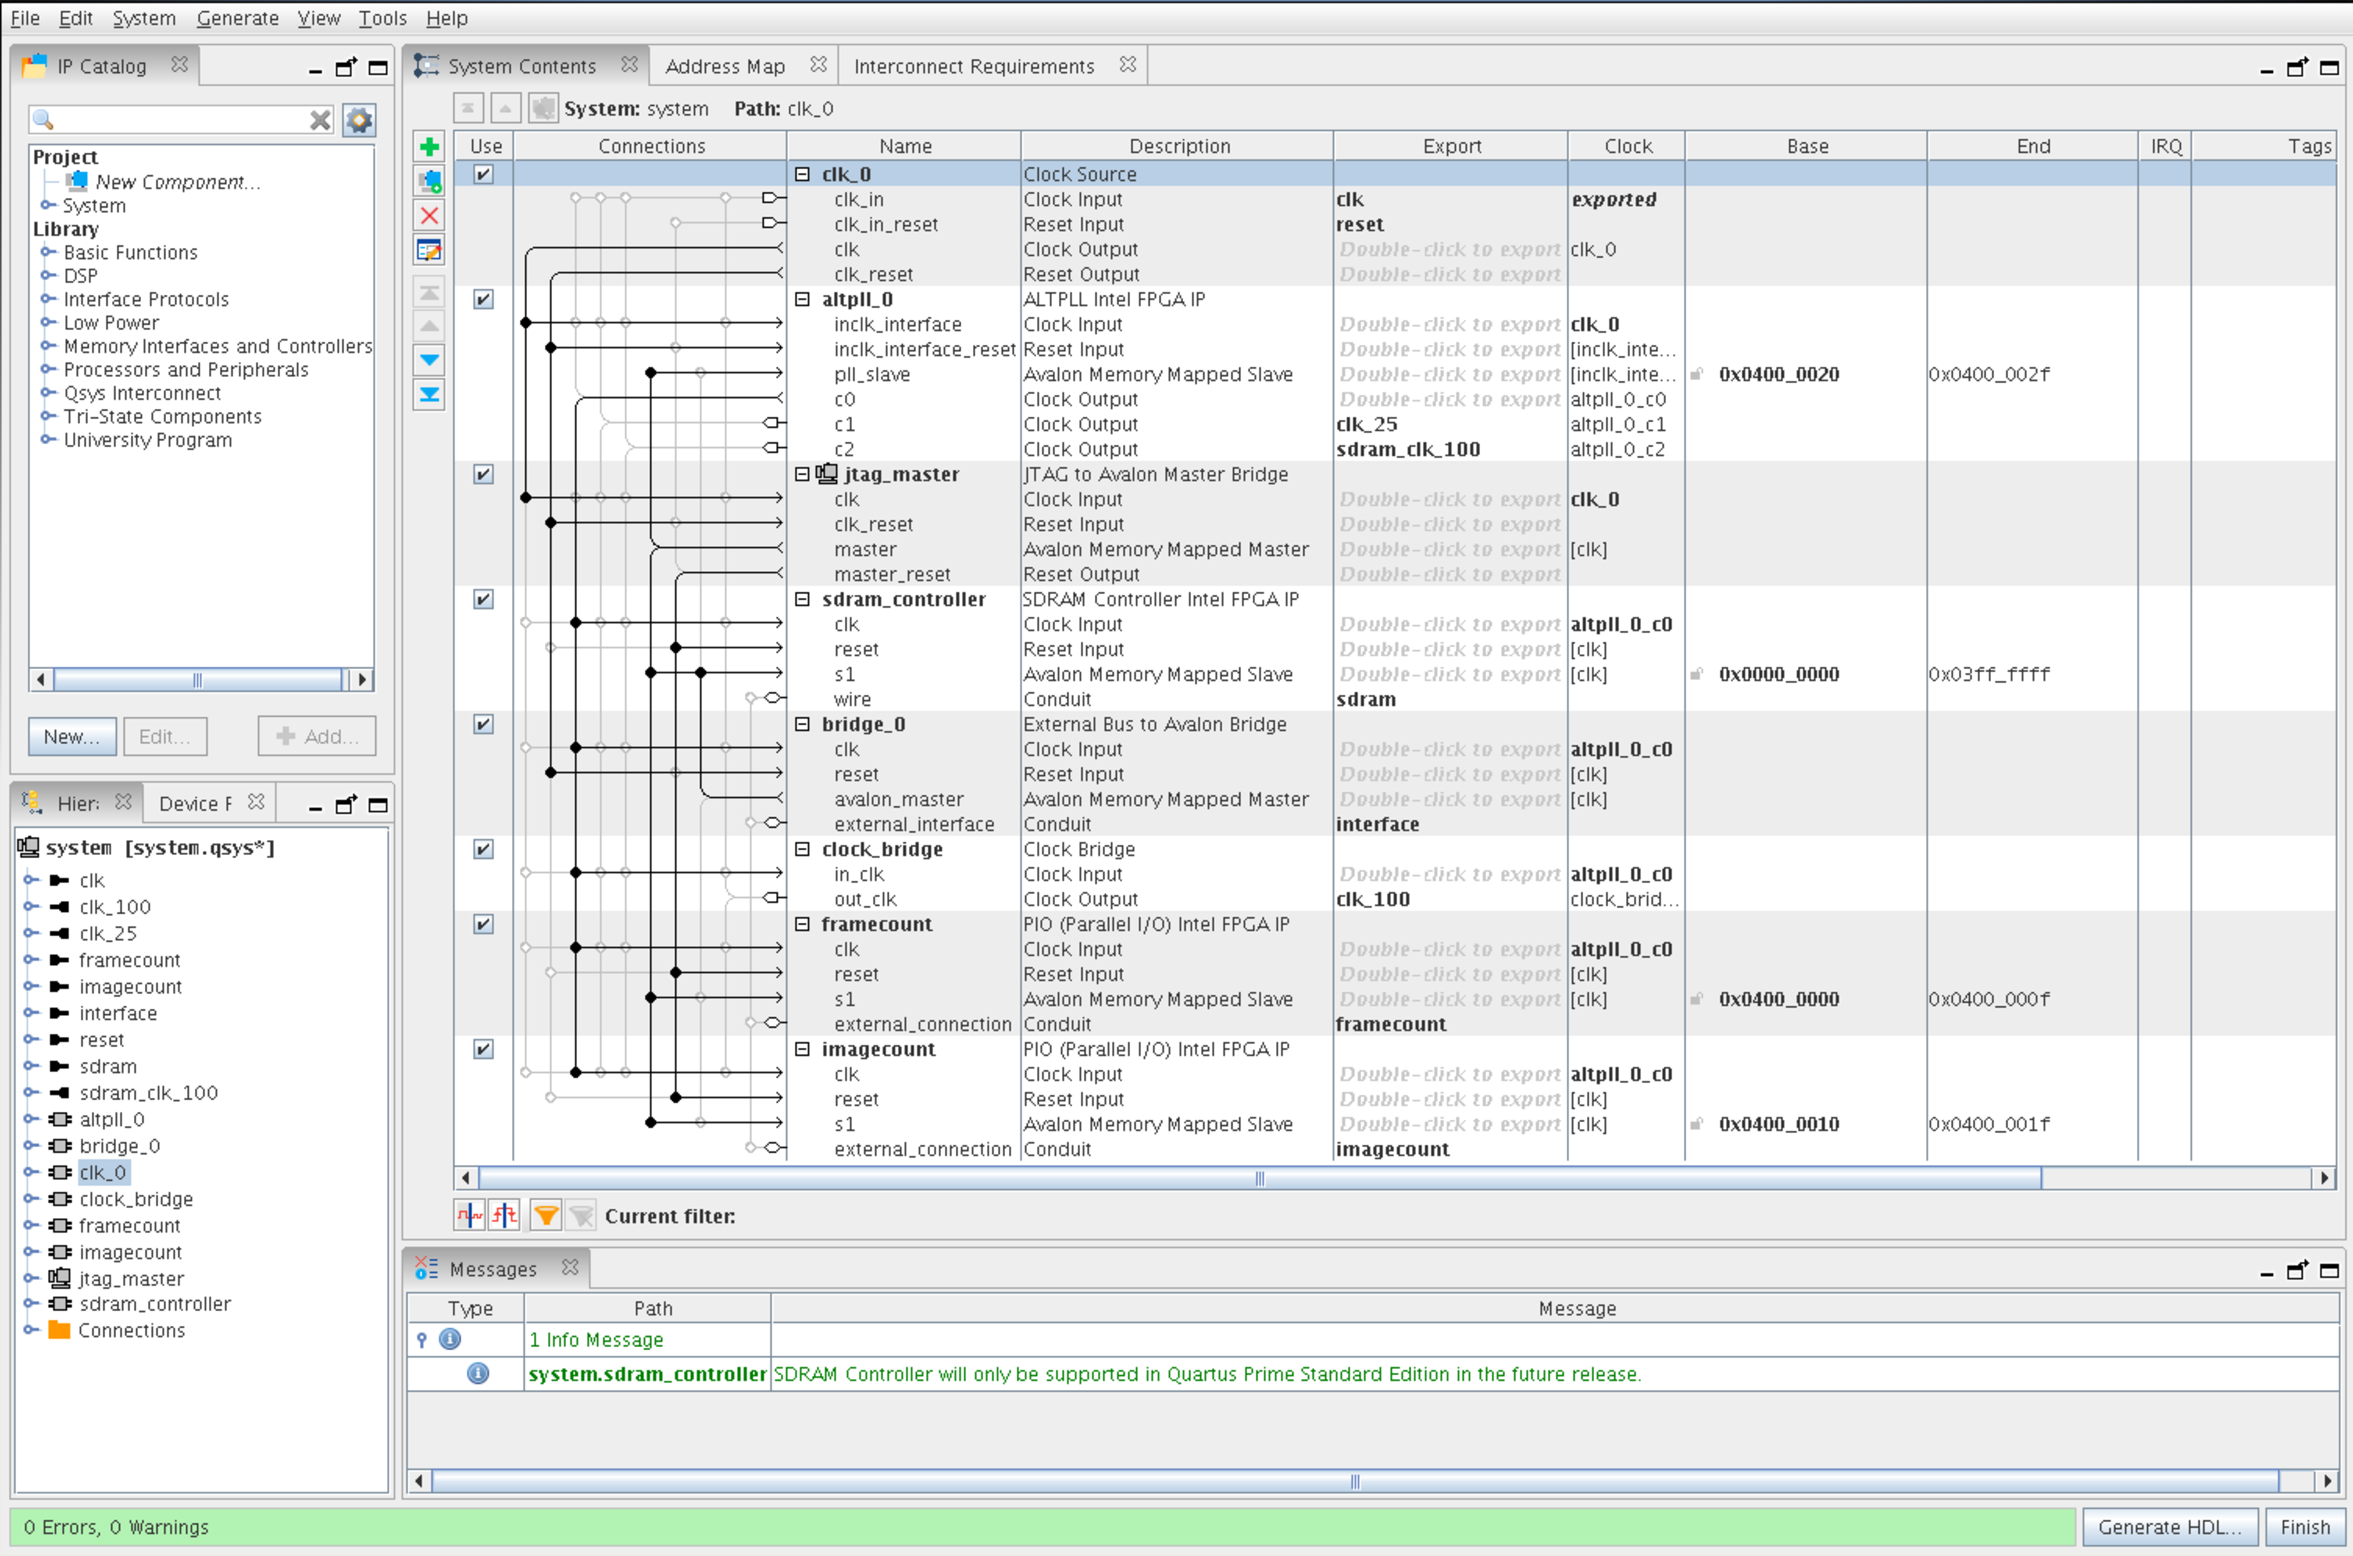
\includegraphics[width=1.0\textwidth]{graphics/platform_designer.pdf}
	\centering\bfseries
	\caption{Play\_gif JTAG Interface System Diagram}
\end{figure}

\end{frame}

\begin{frame}
\frametitle{IP and Platform Designer}

\begin{figure}[h]
	\centering
	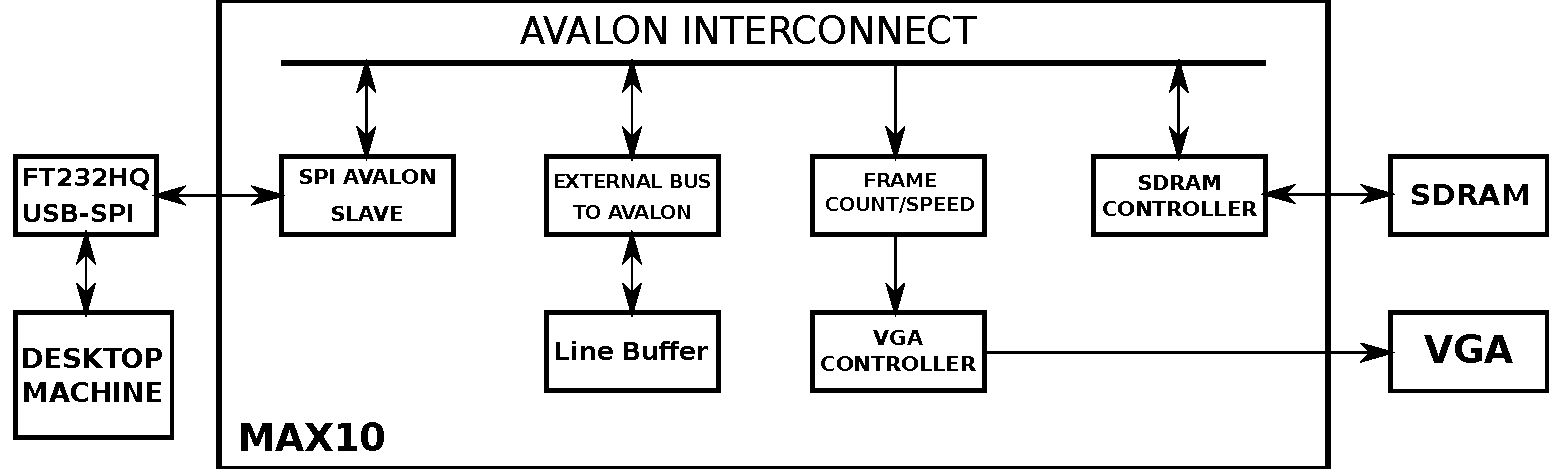
\includegraphics[width=1.0\textwidth]{graphics/spi_avalon_system}
	\centering\bfseries
	\caption{Play\_gif with SPI System Diagram}
\end{figure}

Replacing the JTAG with a SPI interface.  Drop in the included SPI IP!

\end{frame}

\begin{frame}
\frametitle{FTDI USB to SPI Adapter}

The significant change on the FPGA is the swapping of the JTAG Avalon bus master with the SPI-Avalon slave.  This was not entirely a drop-in replacement, as there were changes to reset and clock connections in addition to swapping JTAG to SPI components.  But it is easy, and the swapping can be done in a couple of minutes.

External to the DE10-Lite board, there is a USB to SPI adapter board.  This board is based on the FT232H chip by FTDI.  This can be bought from eBay for about \$10.  Search for ``ft232 spi'' and you will find several options.  I recommend one with headers to allow it to be plugged into a common breadboard.  The FTDI device requires a C shared library (libMPSSE) to be installed:

\url{https://www.ftdichip.com/Support/SoftwareExamples/MPSSE/LibMPSSE-SPI.htm}

\end{frame}

\begin{frame}
\frametitle{DE10-Lite + FTDI USB to SPI}

Here is the rapid-prototype breadboard hook-up:

\begin{figure}[h]
	\centering
	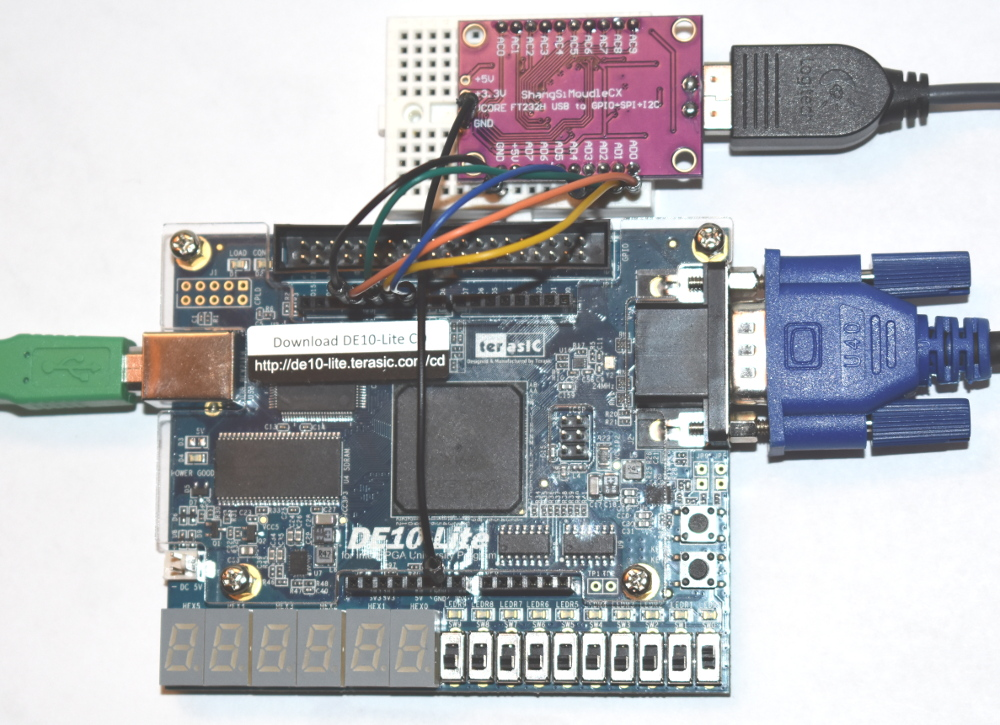
\includegraphics[width=0.5\textwidth]{graphics/de10_spi}
	\centering\bfseries
	\caption{DE10-Lite Connected to FTDI SPI Breakout}
\end{figure}

In spite of the length of the breadboard jumper wires, the SPI interface performed remarkably well right up to the FTDI clock limit of 30 MHz.

\end{frame}

\begin{frame}
\frametitle{SPI Driver in Julia Programming Language}

The github project from which mine was derived uses a programming language called ``Julia'' in the JTAG server and for image data processing:

\begin{figure}[h]
	\centering
	
\includegraphics[width=0.30\textwidth]{graphics/logo}
	\centering\bfseries
	\caption{\url{https://julialang.org/}}
\end{figure}

Rather than reinventing the wheel, I decided to use the image processing portion of the Julia program.
However, how to drive the FTDI SPI device?  I needed something to replace the JTAG server.

\end{frame}

\begin{frame}
\frametitle{SPI Driver in Julia Programming Language}

The FTDI USB-to-SPI device is supported with a C shared library.  This library has the initialization, read, write, and shutdown
command necessary to work with the device.

Fortuitously, the Julia language includes the capability to call C library functions in a very direct way!
I was skeptical at first, but I quickly had the SPI device's initialization function running and returning with no error.
The other required functions were quickly added.  I now had full control of the SPI bus from the command line!

\end{frame}

\begin{frame}
\frametitle{Project System Diagram}

\begin{figure}[h]
	\centering
	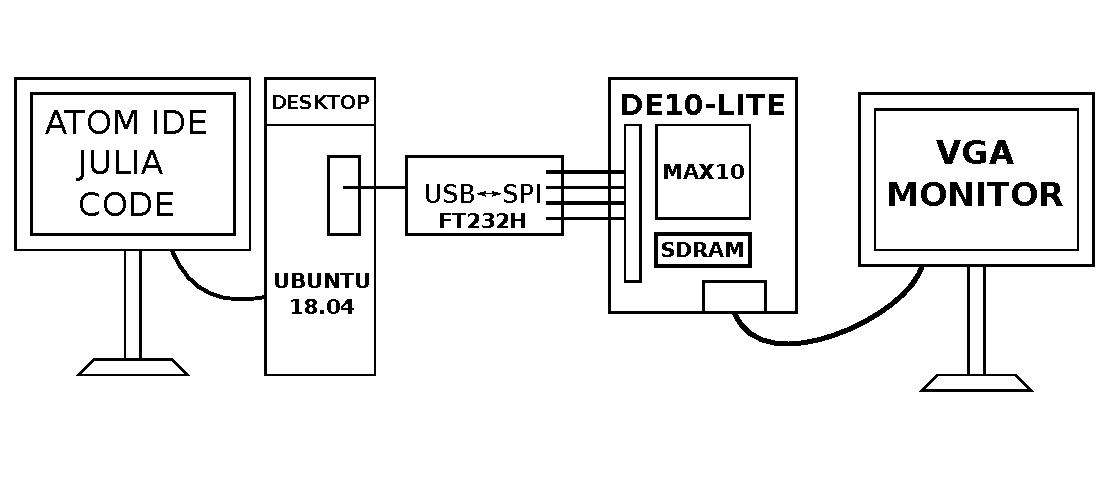
\includegraphics[width=0.95\textwidth]{graphics/project_system}
	\centering\bfseries
	\caption{Project System: Desktop -$>$ USB-to-SPI $<$-$>$ FPGA -$>$ VGA Monitor}
\end{figure}

\end{frame}

\begin{frame}
\frametitle{Notes on Verilog/SystemVerilog}

A good book which costs \$20 at Amazon:

You will need to go up the learning curve on Hardware Description Language.
Here an inexpensive book (\$20) which will get you going:

``Designing Digital Systems with SystemVerilog''
Brent E. Nelson, Brigham Young University

\begin{figure}[h]
	\centering
	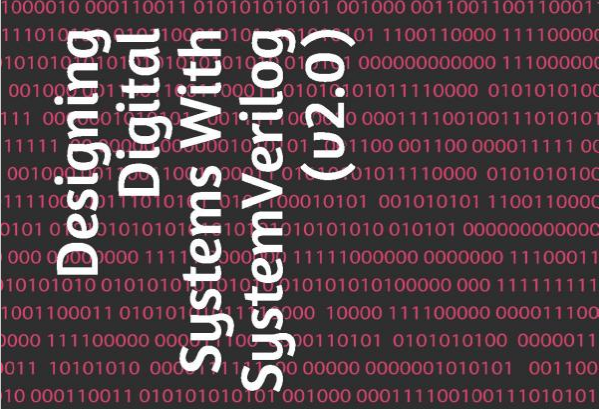
\includegraphics[width=0.60\textwidth]{graphics/systemverilog.png}
	\centering\bfseries
	\caption{``Designing Digital Systems with SystemVerilog'' by Brent Nelson}
\end{figure}
\end{frame}

\begin{frame}
\frametitle{Notes on Verilog/SystemVerilog}

The most important thing to understand about Verilog/SystemVerilog from the Nelson book:

``You must remember that when designing using an HDL (Hardware Description Language), you are not writing a computer program which will be compiled and then executed sequentially like C or Java.  Rather, you are describing a set of hardware building blocks and their interconnections.''

\end{frame}

\begin{frame}
\frametitle{The New Wave of FPGA: Sipeed}

\begin{tiny}
\url{https://www.seeedstudio.com/Sipeed-TANG-PriMER-FPGA-Development-Board-p-2881.html}
\end{tiny}

\begin{figure}[h]
	\centering
	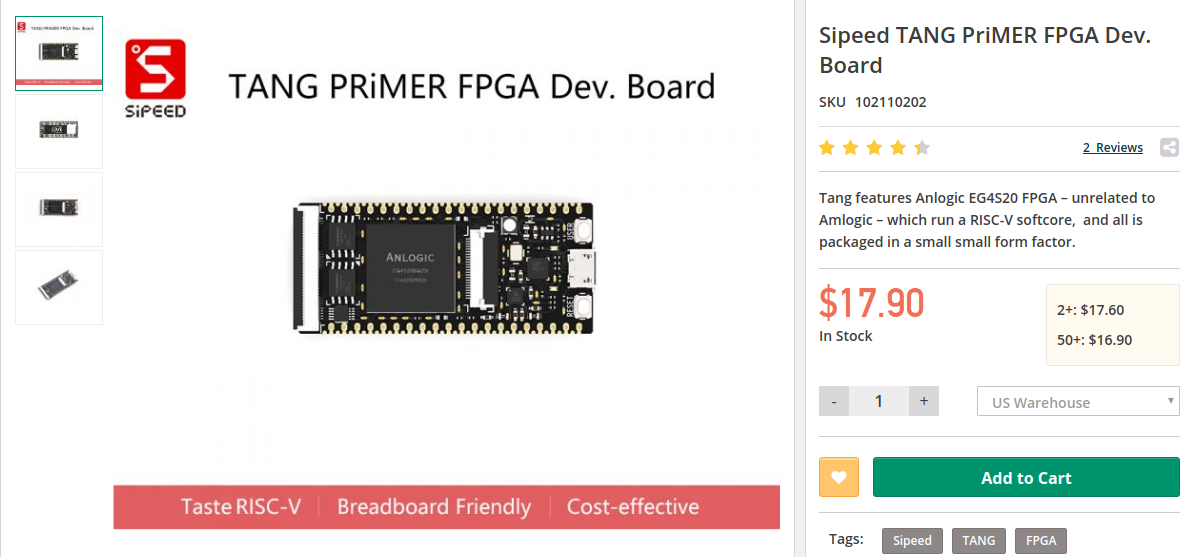
\includegraphics[width=0.95\textwidth]{graphics/sispeed_tang_fpga.png}
	\centering\bfseries
	\caption{Sipeed Tang Primer FPGA Development Board}
\end{figure}

\end{frame}

\begin{frame}
\frametitle{The New Wave of FPGA: Arduino Vidor}

\url{https://store.arduino.cc/usa/mkr-vidor-4000}

\begin{figure}[h]
	\centering
	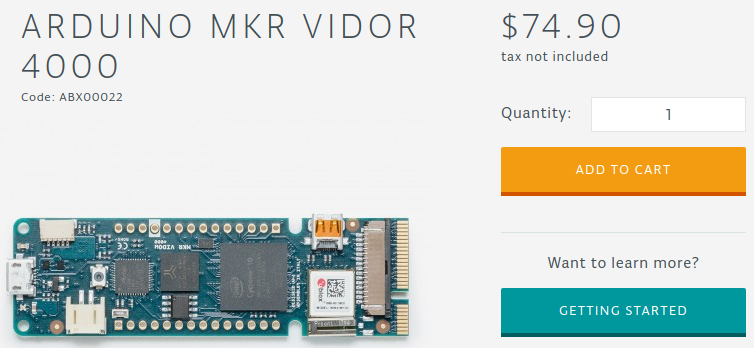
\includegraphics[width=0.95\textwidth]{graphics/arduino_vidor.png}
	\centering\bfseries
	\caption{Arduino Vidor:  Intel Cyclone 10CL016 + Microchip SAMD21 (32 bit ARM Cortex M0+)}
\end{figure}


\end{frame}

\begin{frame}
\frametitle{The New Wave of FPGA: TinyFPGA}

\url{https://www.adafruit.com/product/4038}

\begin{figure}[h]
	\centering
	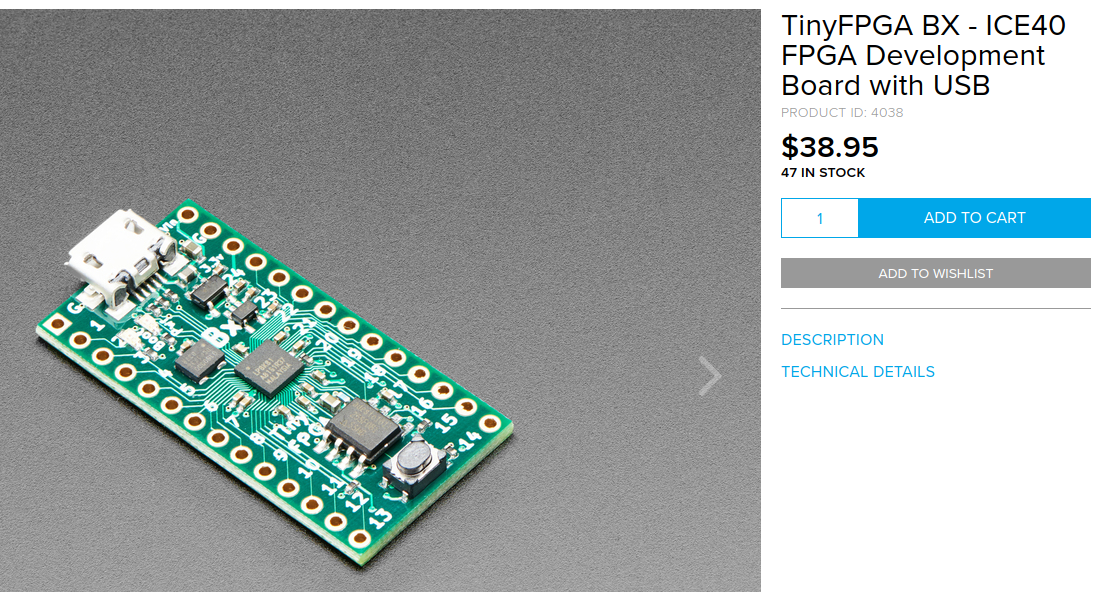
\includegraphics[width=0.95\textwidth]{graphics/tinyfpga.png}
	\centering\bfseries
	\caption{TinyFPGA: Lattice ICE40 FPGA. Supported by open-source tools!}
\end{figure}


\end{frame}

\begin{frame}
\frametitle{Github Repositories}

Github repositories for my FPGA projects:

Conference paper and slides in this one:
\url{https://github.com/Greg-R/spiavalonfpga}

My rotator control project:
\url{https://github.com/Greg-R/rotorcommand1}

\end{frame}

\begin{frame}
\frametitle{FPGAs in the Silicon Ecosystem}

Boiling it down to fundamental capabilities:

\begin{figure}[h]
	\centering
	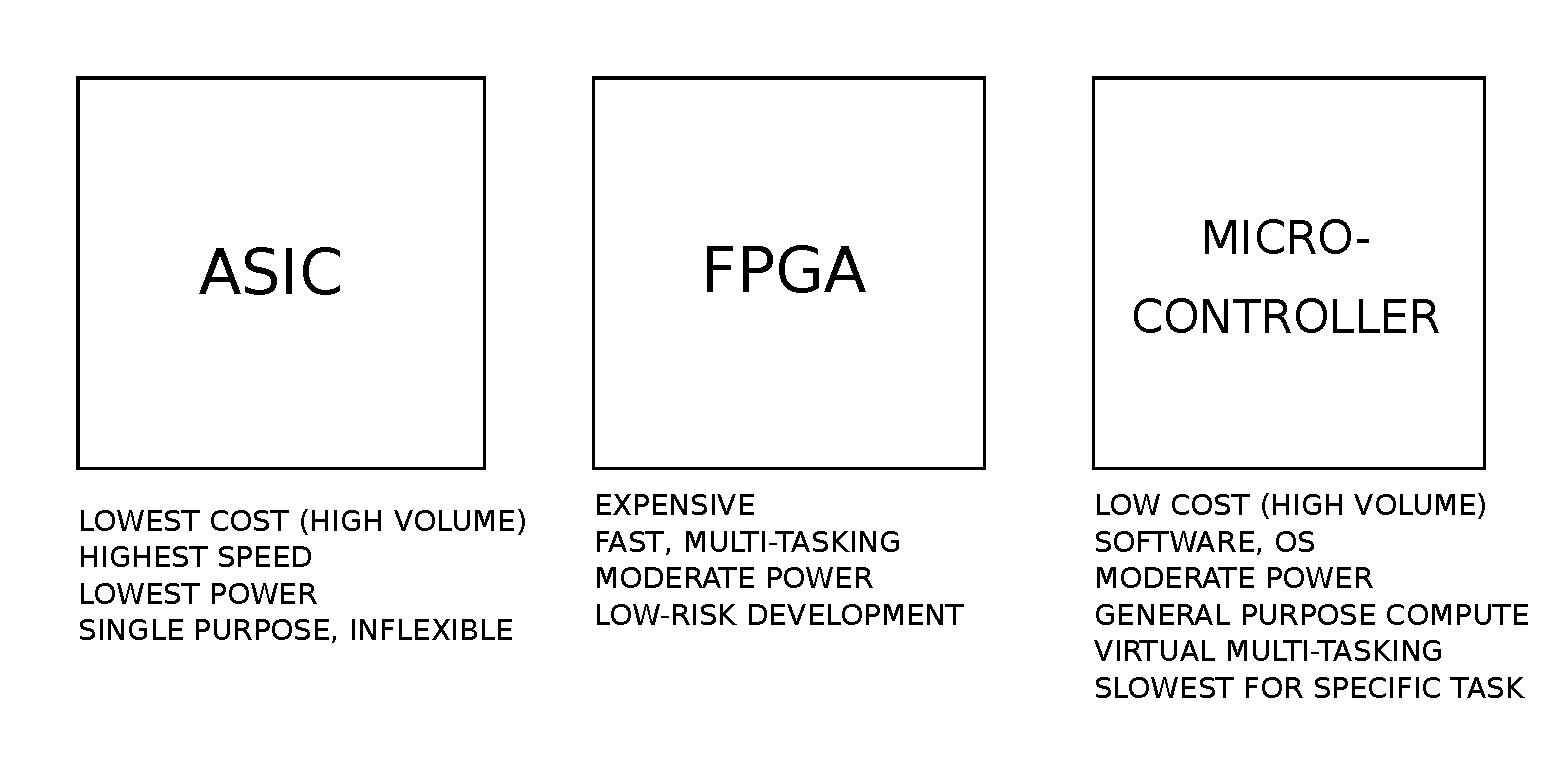
\includegraphics[width=1.0\textwidth]{graphics/asic_fpga_micro}
	\centering\bfseries
	\caption{Digital Hardware in Silicon Comparison}
\end{figure}

\end{frame}

\end{document}
